\documentclass{report}

% Packages for math symbols and equations
\usepackage[T1]{fontenc}
\usepackage[utf8]{inputenc}

\usepackage[margin=1.4in]{geometry}
\usepackage{graphicx}

\usepackage{amssymb,amsthm, amsmath}
%\usepackage{mathtools}
%\numberwithin{equation}{section}

\usepackage[
natbib,
style=alphabetic,
maxbibnames=10,  
sorting=ydnt,
url=false,
doi=false,
sortcites,
defernumbers,
backref,
backend=biber
]{biblatex}
\addbibresource{bibliography.bib}

\usepackage{hyperref}

\usepackage{todonotes}
%\setuptodonotes{inline}
\usepackage{url}

\usepackage[nameinlink, capitalise, noabbrev]{cleveref}

\usepackage{xfrac}
\usepackage{nicefrac}

\usepackage{soul}

\usepackage{bbm}

\usepackage{enumitem}

%For double brackets \llbracket \rrbracket
\usepackage{stmaryrd}

\crefname{assumption}{Assumption}{Assumptions}

\newtheorem{theorem}{Theorem}

\newtheorem{proposition}{Proposition}[section]
\newtheorem{lemma}{Lemma}[section]
\newtheorem{corollary}{Corollary}[section]
\theoremstyle{remark}
\newtheorem{remark}{Remark}[section]


\theoremstyle{definition}
\newtheorem{example}{Example}[section]
\newtheorem{counterexample}{Counterexample}[section]
\newtheorem{definition}{Definition}[section]
\newtheorem{assumption}{Assumption}

%\numberwithin{equation}{section}

%\renewcommand{\baselinestretch}{2}

%\newcounter{hypcounter}

\newcommand{\N}{\mathbb{N}}
\newcommand{\Z}{\mathbb{Z}}
\newcommand{\R}{\mathbb{R}}
%\DeclareMathOperator{\dom}{dom}
\newcommand{\closure}[1]{\overline{#1}}
\newcommand{\norm}[1]{\left\Vert #1 \right\Vert}
\newcommand{\seminorm}[1]{\left[ #1 \right]}
\newcommand{\abs}[1]{\left\vert #1 \right\vert}
%\DeclareMathOperator{\divtmp}{div}
\renewcommand{\div}{\divtmp}
% \DeclareMathOperator{\argmin}{arg\,min}
% \DeclareMathOperator{\argmax}{arg\,max}
% \DeclareMathOperator{\esssup}{ess\,sup}
% \DeclareMathOperator{\essinf}{ess\,inf}
\renewcommand{\st}{\,:\,}
% \DeclareMathOperator{\supp}{supp}
\newcommand{\dx}{\,\mathrm{d}x}
\renewcommand{\d}{\,\mathrm{d}}
\newcommand{\dH}{\,\mathrm{d}\mathcal{H}^{n-1}(x)}
% \DeclareMathOperator{\sign}{sign}
\newcommand{\eps}{\varepsilon}
% \DeclareMathOperator{\dist}{dist}
% \DeclareMathOperator{\Lip}{Lip}
\newcommand{\KR}{\mathrm{KR}}
\newcommand{\C}{\mathrm{C}}
\renewcommand{\L}{\mathrm{L}}
\newcommand{\W}{\mathrm{W}}
\newcommand{\M}{\mathcal M}
\newcommand{\grad}{\nabla}
\newcommand{\hess}{\mathrm{D}^2}
\newcommand{\defeq}{:=}
% \DeclareMathOperator{\diam}{diam}
\newcommand{\Set}[1]{\left\lbrace#1\right\rbrace}
\newcommand{\scale}{\eps}
\newcommand{\res}{\delta}


\newcommand{\wto}{\rightharpoonup}
\newcommand{\wsto}{\overset{\ast}{\rightharpoonup}}
\newcommand{\strictto}{\overset{\mathrm{str}}{\rightharpoonup}}

\newcommand{\rev}{\color{magenta}}
\renewcommand{\rev}{}
\newcommand{\red}{\color{red}}
\newcommand{\blue}{\color{blue}}
\newcommand{\nc}{\normalcolor}


% Lie math operators
\DeclareMathOperator{\toledo}{T}
\DeclareMathOperator{\isom}{Isom}
\DeclareMathOperator{\bus}{b}
\DeclareMathOperator{\ii}{i}
\DeclareMathOperator{\spa}{span}
\DeclareMathOperator{\class}{C}
\DeclareMathOperator{\diam}{diam}
\DeclareMathOperator{\diag}{diag}
\DeclareMathOperator{\U}{{\mathrm{U}}}
\DeclareMathOperator{\SL}{{\mathrm{SL}}}
\DeclareMathOperator{\SU}{{\mathrm{SU}}}
\DeclareMathOperator{\su}{{\mathfrak{su}}}
\DeclareMathOperator{\PSL}{{\mathrm{PSL}}}
\DeclareMathOperator{\GL}{{\mathrm{GL}}}
\DeclareMathOperator{\SO}{{\mathrm{SO}}}
\DeclareMathOperator{\PGL}{{\mathrm{PGL}}}
\DeclareMathOperator{\PO}{{\mathrm{PO}}}
\DeclareMathOperator{\PSO}{{\mathrm{PSO}}}
\DeclareMathOperator{\id}{id}
\DeclareMathOperator{\inte}{int}
\DeclareMathOperator{\LC}{LC{}}
\DeclareMathOperator{\F}{Frenet{}}
\DeclareMathOperator{\lie}{Lie}
\DeclareMathOperator{\Ker}{Ker}
\DeclareMathOperator{\ad}{ad}
\DeclareMathOperator{\Hff}{dim_{Hf{}f}}
\DeclareMathOperator{\vol}{Vol}
\DeclareMathOperator{\rk}{rank}
%\DeclareMathOperator{\jac}{jac}
\DeclareMathOperator{\gap}{{\sf{gap}}}
\DeclareMathOperator{\ann}{Ann}
\DeclareMathOperator{\Ad}{Ad}

\newcommand{\restr}{\mathbin{\vrule height 1.6ex depth 0pt width
0.13ex\vrule height 0.13ex depth 0pt width 1.3ex}}

% Title page information
\title{Limit sets of Anosov representations}
\author{Giorgos}
\date{\today}

\begin{document}

\maketitle

\tableofcontents

\chapter{Introduction}
\begin{definition}
For $p \in \{2, \ldots, d\}, s\in \mathbb R $
and $g \in SL(d, \mathbb R)$ 
we denote with $\Psi_s^p(g): \mathfrak a ^+ \to \mathbb R$ the functional:
\begin{align*}
\Psi_s^p(g) &= 
    \alpha_{12}(a(g)) + \cdots + \alpha_{1(p-1)}(a(g)) + (s - (p-2))\alpha_{1p}(a(g))\\
\tilde \Psi_s^p(g) &= 
    \left( \frac{\sigma_2}{\sigma_1}\cdots\frac{\sigma_{p-1}}{\sigma_1}(g)\right) 
    \left( \frac{\sigma_{p-1}}{\sigma_1}(g) \right)^{s - (p-2)}
\end{align*}
\end{definition}
\begin{remark}
    We have $\alpha_{ij}(a) = a_i - a_j, a_i(g) = \log (\sigma_i(g))$ and 
    \[
        \Psi_s^p(g) = \log \tilde \Psi_s^p(g)
    \]
and that
\begin{align*}
    \min_{p \in \llbracket 2, d \rrbracket} 
    \left\{ 
        \sum_{|\gamma| = T} 
            \frac{\sigma_2}{\sigma_1}\cdots\frac{\sigma_{p-1}}{\sigma_1}(g) 
            \left( \frac{\sigma_{p-1}}{\sigma_1}(g) \right)^{s - (p-2)}
    \right\} = 
    \sum_{|\gamma| = T} e^{-\max\limits_{p \in \llbracket 2, d \rrbracket} \Psi_s^p(g)}
\end{align*}
\end{remark}

The following definition comes from \cite{ledrappier_dimension_2023}, in the special case of projective Anosov representations ($P = {1}$):
\begin{definition}
    For $s \geq 0$ we consider the Falconer functional $F_s : \SL(d, \mathbb R) \to \mathbb R$ by:
    \[
        F_s(g) = \min 
        \left\{
            \sum_{j=2}^d s_j \alpha_{1j}(a(g)) : s_j \in (0,1], \sum_{j=2}^d s_j = s 
        \right\}
    \]
\end{definition}

\begin{remark}
    Using elementary computations one may prove that for all $s \geq 0$:
    \[
        F_s(g) = \min_{p \in \llbracket 2, d \rrbracket} \Psi_s^p(g)
    \]
\end{remark}
\chapter{Upper bound}
\begin{lemma}[Upper bound for dimension]
Let $\rho: \Gamma \to \SL(d, \mathbb R)$ be a projective Anosov representation. 

\[
    \dim_H(\xi^1 (\partial \Gamma) ) \leq
    \inf 
    \left\{ 
        s :  
        \sum_{|\gamma| = T} e^{-\max\limits_{p \in \llbracket 2, d \rrbracket} \Psi_s^p(\rho(\gamma))}  < \infty
    \right\}
\]
\end{lemma}

The following can be found in \cite[Proposition 3.3]{pozzetti_anosov_2023}:
\begin{proposition}
    Let $\rho: \Gamma \to SL(d, mathbb R)$ be projective Anosov and $\alpha > 0$
    Then there exist $c_0, c_1 > 0$ that depends only on $\alpha$ and $\rho$ such that for all $\gamma \in \Gamma$:
    \[
        (\xi^1)^{-1}(B_{\alpha_1, \alpha}(\rho(\gamma))) \subseteq C_{c_0,c_1}^\infty(\gamma)
    \]
\end{proposition}
\begin{proof}
    We begin by noting that it suffices to show this for all but finitely many $\gamma \in \Gamma$, since then we may alter the constants to satisfy the wanted inclusion also for the finitely many remaining $\gamma \in \Gamma$. Given this, we shall assume that $|\gamma| \geq l_0$ where $l_0 > 0$ is such that $Ce^{-\mu l_0} < 1$ and $C, \mu > 0$ are the constants appearing in the definition of the Anosov property of $\rho$..

    Suppose $x \in \partial \Gamma$ such that $\xi^1(x) \in B_{\alpha_1, \alpha}(\rho(\gamma))$, and consider a geodesic ray $a_j \to x$ starting from $a_0 = e$.
    To prove the result, it suffices to find constants $c_0, c_1$ independent of $\gamma$ and a ($c_0$, $c_1$)-quasi-geodesic from $\gamma^{-1}$ to $x$ that passes through $e$ and stays at a bounded distance from $(a_j)_{j=0}^\infty$

    Using \cite[Proposition 2.5]{pozzetti_anosov_2023} we have that
    $d(\xi^1(a_j), U_{d-1}(\rho(\gamma^{-1}))) \leq C e^{-\mu j}$, 
    so there exists some $L>0$ that depends only on $\alpha$ 
    such that for all $j\geq L: U_1(\rho(a_j))\in B_{\alpha_1, \alpha}(\rho(\gamma))$ and in particular
    \[
        d(\xi^1(a_j), \gamma^{-1}) = d(U_1(\rho(a_j)), U_1(\rho(\gamma^{-1}))) \geq 
        d(U_1(\rho(a_j)), U_{d-1}(\rho(\gamma^{-1}))) > \sin\alpha.
    \]
    Along with the uniform continuity of $\xi^1: \Gamma \cup \partial \Gamma \to \mathbb P(\mathbb R^d)$ this implies there exists some $\alpha' > 0$ and $L>0$ such that for all $j\geq L$:
    \[
        d(a_j, \gamma^{-1}) \geq \alpha'.
    \]
    Upon considering a large $L$, we may also assume that $|a_L| = L > l_0$. Note that both $\alpha'$ and $L$ do not depend on each $\gamma$ but only on $\rho$ and $\alpha$.

    Using some geometric group theory, we can show that for all $j \geq L$
    \[
        d(\gamma^{-1}, a_j) > \alpha' \Rightarrow
        d([\gamma^{-1}, a_j], e) < \alpha''
    \]
    for some $\alpha''$ that depends only on $\Gamma$ and $\alpha'$, where $[a_j, \gamma^{-1}]$ denotes the geodesic segment connecting $\gamma^{-1}$ and $a_j$.

    Consider the concatenation $(a_j')_{j=L-K}^\infty$ of $[\gamma^{-1},a_L]$ and $[a_L, x]$.
    To find quasi-geodesic-constants that are uniform in $\gamma$, we note that for any $c_0 \geq 1, c_1 \geq 0$:
    \[
        c_0^{-1} |i - j| - c_1 \leq d(a_i', a_j') = d(a_i, a_j) \leq d(a_i) c_0^ |i - j| + c_1 
        \text{ when } i,j \geq L \text{ or } i,j \leq L
    \]
    and that the upper bound follows trivially by the triangle inequality. 
    
    For the lower bound we proceed in two steps. 
    First we bound the distance of $\gamma^-1 = a_{L-K}'$ to $a_{L+j}$ for $j\geq 0$:
    \begin{align*}
        d(a_{L-K}', a_{L+j}') 
        &\geq \nu (|a_{L+j}| - |\gamma^{-1}|) - c_0' -c_1'|\log(d(U_1(\rho(a_{L+j})), U_1(\rho(\gamma^{-1}))))| \geq\\
        &\geq \nu((L+j) + (K-L)) - c_0' -c_1'|\log(\sin a)| \geq\\
        &= c_0^{-1} (j+K) - c_1
    \end{align*}
    for $c_0 = \nu^{-1}, c_1 = c_0' + c_1'|\log(\sin \alpha)|$.
    The first inequality comes from \cite[Lemma 3.9]{pozzetti_anosov_2023}. For the second inequality we estimate $|\gamma^{-1}|$ from below using the triangle inequality.
    We are now ready to show that the concatenation $(a_j')_j$ is indeed a ($c_0$, $c_1$)-geodesic:
    \begin{align*}
        d(a_{L+j}, a_{L-i}) &\geq d(a_{L+j},a_{L_K}) - d(a_{L_K}, a_{L-i}) \geq
        c_0^{-1} (j+K) - c_1 - (K - i) \geq\\
        &\geq c_0^{-1} (j+i) - c_1.
    \end{align*}

    Note however that $(a_j')$ does not necessarily lie in $C_\infty^{c_0, c_1}$ since it may not pass through $e$.
    For this reason we some $L - K \leq i_0\leq L$ such that $|a_{i_0}| < \alpha''$, the existence of which is guaranteed by the fact that $d([\gamma^{-1}, a_L], \epsilon) < \alpha''$.
    We then consider alter $(a_j')$ at $i_0$ so that it passes through $e$ to obtain 
    \begin{align*}
        a_j''=
        \begin{cases}
            a_j & \text{for } j\neq i_0 \\
            e & \text{for } j = i_0
        \end{cases}      
    \end{align*}
    which is a ($c_0, c_1 + \alpha''$)-quasigeodesic passing from $e$ and converging to $x$.
\end{proof}
\begin{figure}[h]
    \centering
    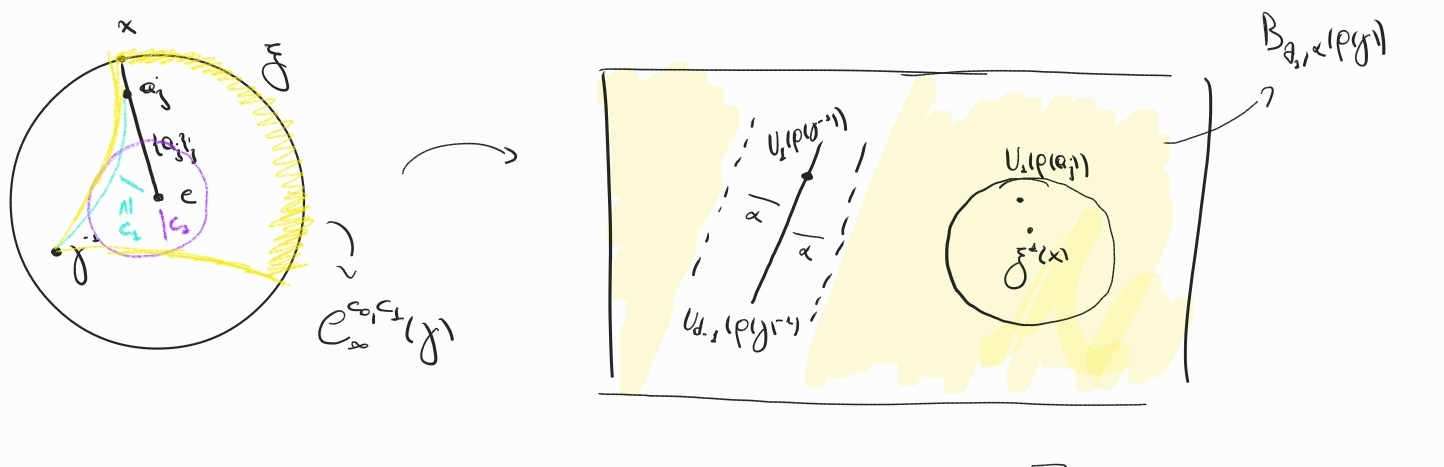
\includegraphics[width=0.8\textwidth]{cone.jpg}
\end{figure}    
\printbibliography

\end{document}